%!TEX ROOT = ./main.tex

\section{Experimental Evaluation}\label{sec:experiments}
%\MS{List the specifications of the cluster machine/laptop with which we have run our experiments.}
We evaluate a prototype implementation of ALg.~\ref{alg:abcd-for-tracking}
on two examples. 
The design of nominal controller has been performed on a laptop with core i7-4510u CPU at 3.10GHz, with 8GB of
RAM.
The formal controller synthesis has been performed
on a cluster with 4 Intel Xeon E7-8857 v2 CPUs (48 cores in total) at 3GHz, with 1.5TB of
RAM.

%\textcolor{red}{
\subsection{Unicycle example}\label{sec:MultiAgent}
In this example, we are focusing on number of robots. This example consist of 10 identical unicycle model . Each unicycle should start from own initial point and reach target set which is shown in Fig. \ref{fig:MA} with green points and red points. while it avoids obstacles and collision with other agents. Unicycle model is described in below.
\begin{equation}\label{eq:unicycle_ss}
	f^{u}(x(t),u(t))=
	\begin{bmatrix}
	\dot{x_1}\\
	\dot{x_2}\\
	\dot{x_3}
	\end{bmatrix}=
	\begin{bmatrix}
	u_1cos(x_3)\\
	u_1sin(x_3)\\
	u_2
	\end{bmatrix}.
\end{equation}
In Eq. \ref{eq:unicycle_ss} $u_1$ is linear speed and $u_2$ is  angular speed and $x_1$ and $x_2$ represents positions and $x_3$ is the angle. Here goal of the problem is designing a controller which satisfy the specifications which mentioned in sec. \ref{sec:Problem_statement}. For this purpose, According to sec.\ref{sec:nominal trajectory} at first we combine all of unicycle dynamics to create a centralized model of the centralized system. The centralized system has $10\times3$ dimension for state space and $10\times2$ dimension for input space. For collision avoidance and obstacle avoidance we use $\delta_{col}=1.5$ and $\delta_{obs}=2$ and we use euclidean distance as a metric for distance in 2D space. In this step, we solved mentioned problem with ALTRO with sample time 0.05 and 200 points for trajectory. Computation takes 138 seconds. Result of ALTRO is illustrated in fig \ref{fig:MA}. 
In next step we synthesize close loop controller using ABCD with $\varepsilon=[0.16,0.16,0.16]$. As we mentioned in Prob. \ref{alg:abcd-with-time-for-tracking} we are going to to design a controller that is able to track the trajectory with $\varepsilon$ distance in every time step which is also robust to the disturbance .\MZ{Here we can split the centralized system to 10 separate system and design a close loop controller for each one of them separately.} In order to do this step, we select $\varepsilon$ in a way that it satisfies $\delta_{col} > 2\sqrt{\varepsilon_x^2+\varepsilon_y^2}$ (since tubes should not intersect with each other). Then we are able to design a controller guaranteeing the specifications for each agent independently using Alg. \ref{alg:abcd-with-time-for-tracking} and SCOTS. We select parameters in this way:\\
$\widetilde{X}=[-1:11]*[-1:11]*[-\pi,\pi]*[0,1]$\\
$U=[-3,3]*[-3,3]$\\
$\eta_{\widetilde{X}}=[0.04,0.04,0.04,0.05]$\\
$\eta_{U}=[0.6,0.6]$\\
number of states = about $7*10^7$\\
reduced number of states = about $7*10^7$\\
number of inputs =121\\

Abstraction in total for 10 systems takes about 12 minutes(average 100 seconds for each system) and synthesizing controller takes about 2 minutes(near 15 seconds for each system). Controller designed in this way is able to overcome bounded additive disturbance $|w|\leq[0.03,0.03,0.03]$ (for all of unicycles). Nominal controller which is produced by ALTRO with presence of this disturbance will be pushed outside of $\epsilon$ tube and also as it shown in the Fig.\ref{fig:MA}, trajectory 1 and 2 will have collision with this value of disturbance. 
\begin{figure}[t]\label{fig:MA}
	\centering
	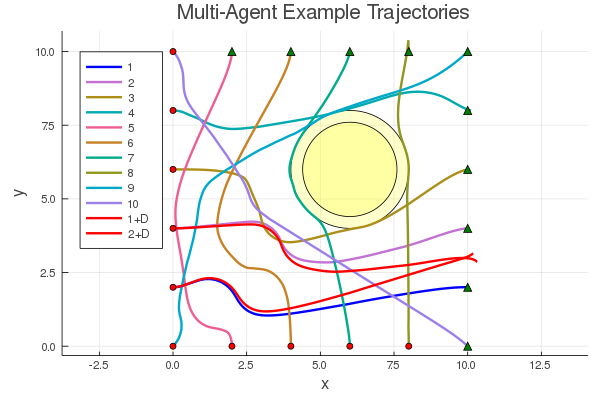
\includegraphics[width=0.85\textwidth]{figures/MA.png}
	\caption{Nominal trajectories of unicycles produced by ALTRO .}
\end{figure}




 %Figure~\ref{fig:inv_pend} demonstrates variations of disturbance limit under which SCOTS is able to find a controller for different tube width. %It can be observed that by increasing the tube width, SCOTS is able to synthesize a controller for larger disturbance levels. Figure~\ref{fig:invpend_traj} demonstartes trajectories of the system  \eqref{eq:inv_pend_ssq} governed by controllers synthesized by ALTRO and SCOTS under appliance of constant disturbance vector \MS{$[??,??]$}. As expected, the controller designed by ALTRO is not able to tackle disturbance, while using the controller generated by SCOTS, the trajectory remains within the desired bound.

%\begin{figure}\label{fig:inv_pend}
%	\includegraphics[]{}
%	\caption{Variations of disturbance limit for which SCOTS is able to find a controller with tube size}
%\end{figure}
%\begin{figure}\label{fig:invpend_traj}
%	\includegraphics[]{}
%	\caption{}
%\end{figure}
%\textcolor{red}{
\subsection{Crane and Lifter}
In this example, we show the method can handle multiple heterogeneous dynamical systems. This example is Modelling a special situation in a factory(shown in fig \ref{fig:cr_and_lft}) . Assume there is a crane and and a lifter. Each one of them should reach their destination without having any accident(satisfying specs). The Crane position will change from 0 to 5 and the lifter from 9 to 4.  Here we model the lifter using $\begin{bmatrix} \dot{x_1}\\ \dot{x_2} \end{bmatrix}=\begin{bmatrix} x_2\\ u \end{bmatrix}$ ($x_1$ and $x_2$ are representing position and velocity) and for the crane we use inverted pendulum model with exactly same configuration in \cite{barto1983neuronlike}: \\ 
\[\begin{bmatrix}
\dot{x}\\
\Ddot{x}\\
\dot{\theta}\\
\Ddot{\theta}
\end{bmatrix}=\begin{bmatrix}
\dot{x_1}\\
\dot{x_2}\\
\dot{x_3}\\
\dot{x_4}
\end{bmatrix}=\begin{bmatrix}
x_2\\
g(x_3,x_4,u)\\
x_4\\
f(x_3,x_4,u)\\
\end{bmatrix}\]

where $x$ represent position of the cart  and $\theta$ is angle of the pole, f and g are non-linear functions. The process of controller design is similar to Sec. \ref{sec:MultiAgent}; At first we find a nominal trajectory with ALTRO with required specifications then we robustifing it using our method with modified ABCD.\\
In this example we do not have any static obstacle, but for collision avoidance we use euclidean distance as the metric with $\delta=0.4$ for measuring distance between crane and lifter. We consider hook of crane as a point mass with a radius and lifter as several point mass on circumference of it, So we consider minimum distance between the hook and points of the lifter as the distance. ALTRO solve this trajectory generation problem using sampling time =0.1 and number of points=40 in 10.7 seconds.\\
to guarantee collision avoidance specification we should select tube sizes to satisfy:
\[ \delta_{col}> \varepsilon_x + l*\varepsilon_\theta + \varepsilon^\prime_x\]
where $\varepsilon_x$ and $\varepsilon_\theta$ are tube sizes for position and angle in crane model (cart pole) and l is the length of the joint and $\varepsilon^\prime_x$ is tube size for position of the lifter.
In next phase we use finite abstraction with $\varepsilon_x=9*0.015$ and $\varepsilon_\theta=11*0.015$ and $\varepsilon^\prime_x=9*0.015$. It takes about 1000 seconds for crane (cart-pole system) with (1.15)*($10^{11}$) number of input-states pairs and ($7*10^6$)*(71) reduced number of states and synthesis takes 35 seconds. For lifter abstractions abstraction and synthesis will finish in less than a second.\\
The nominal controller with disturbances $w_1=[0,0.02,0,0]$ for crane and $w_2=[0,0.1]$ for lifter will fail collision specification.


\begin{figure}[t]\label{fig:cr_and_lft}
	\centering
	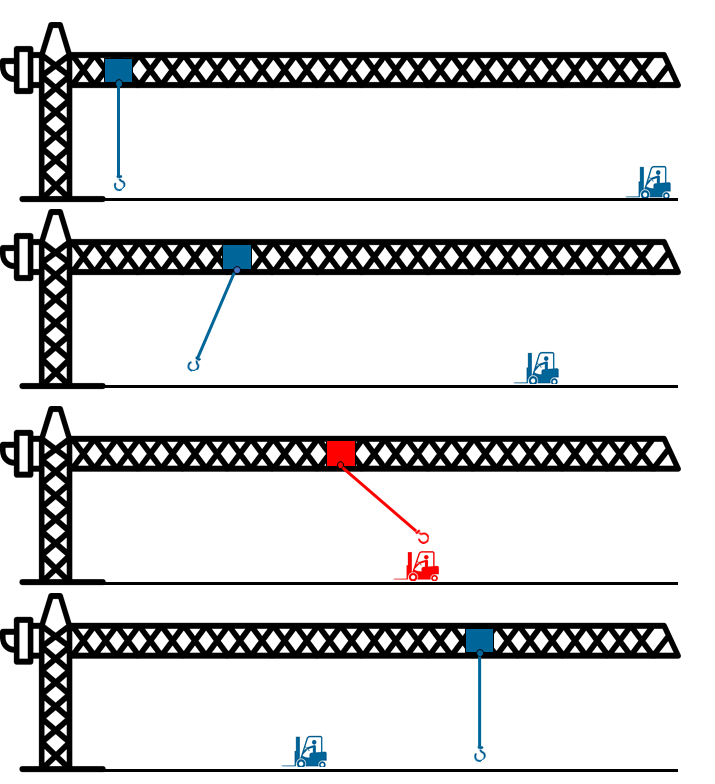
\includegraphics[width=0.85\textwidth]{figures/crane_and_lifter.png}
	\caption{Crane and Lifter example .}
\end{figure}

%} 



\section{Present Challenges}

\begin{enumerate}
	\item In some examples, it was necessary to consider a larger control input space for the SCOTS part, than what was used in the ALTRO part.
	Otherwise, the SCOTS would not be able to track the nominal trajectory within the given precision using any level of discretization. 
	\item For the ship example, applying the largest disturbance with which SCOTS is able to compute a controller, the trajectory resulted from using the open loop controller does not leave  $\varepsilon-$tube around it; in general magnitude of disturbance for which SCOTS can find a controller is relatively small for most of examples that we have tried.
\end{enumerate}




